\documentclass{beamer}


\usepackage{amssymb,amsmath}
\usepackage{graphicx}
\usepackage{url}
\usepackage{color}
\usepackage{relsize}		% For \smaller
\usepackage{url}			% For \url
\usepackage{epstopdf}	% Included EPS files automatically converted to PDF to include with pdflatex

%For MindMaps
% \usepackage{tikz}%
% \usetikzlibrary{mindmap,trees,arrows}%

%%% Color Definitions %%%%%%%%%%%%%%%%%%%%%%%%%%%%%%%%%%%%%%%%%%%%%%%%%%%%%%%%%
%\definecolor{bordercol}{RGB}{40,40,40}
%\definecolor{headercol1}{RGB}{186,215,230}
%\definecolor{headercol2}{RGB}{80,80,80}
%\definecolor{headerfontcol}{RGB}{0,0,0}
%\definecolor{boxcolor}{RGB}{186,215,230}

%%% Save space in lists. Use this after the opening of the list %%%%%%%%%%%%%%%%
%\newcommand{\compresslist}{
%	\setlength{\itemsep}{1pt}
%	\setlength{\parskip}{0pt}
%	\setlength{\parsep}{0pt}
%}

%\setbeameroption{show notes on top}

% You should run 'pdflatex' TWICE, because of TOC issues.

% Rename this file.  A common temptation for first-time slide makers
% is to name it something like ``my_talk.tex'' or
% ``john_doe_talk.tex'' or even ``discrete_math_seminar_talk.tex''.
% You really won't like any of these titles the second time you give a
% talk.  Try naming your tex file something more descriptive, like
% ``riemann_hypothesis_short_proof_talk.tex''.  Even better (in case
% you recycle 99% of a talk, but still want to change a little, and
% retain copies of each), how about
% ``riemann_hypothesis_short_proof_MIT-Colloquium.2000-01-01.tex''?

\mode<presentation>
{
  % A tip: pick a theme you like first, and THEN modify the color theme, and then add math content.
  % Warsaw is the theme selected by default in Beamer's installation sample files.

  %%%%%%%%%%%%%%%%%%%%%%%%%%%% THEME
  %\usetheme{AnnArbor}
  %\usetheme{Antibes}
  %\usetheme{Bergen}
  %\usetheme{Berkeley}		% bem bacana - menu esquerdo
  %\usetheme{Berlin}
  %\usetheme{Boadilla}
  %\usetheme{boxes}
  %\usetheme{CambridgeUS}		% bem bacana - menu superior
  %\usetheme{Copenhagen}
  %\usetheme{Darmstadt}
  %\usetheme{default}
  %\usetheme{Dresden}
  \usetheme{Frankfurt}
  %\usetheme{Goettingen}
  %\usetheme{Hannover}		% bem bacana - menu esquerdo
  %\usetheme{Ilmenau}
  %\usetheme{JuanLesPins}
  %\usetheme{Luebeck}
  %\usetheme{Madrid}		%bacana
  %\usetheme{Malmoe}
  %\usetheme{Marburg}		% bem bacana - menu direito
  %\usetheme{Montpellier}
  %\usetheme{PaloAlto}		% bem bacana - menu esquerdo
  %\usetheme{Pittsburgh}
  %\usetheme{Rochester}		%bacana
  %\usetheme{Singapore}
  %\usetheme{Szeged}
  %\usetheme{Warsaw}

  %%%%%%%%%%%%%%%%%%%%%%%%%%%% COLOR THEME
  %\usecolortheme{albatross}		% azul escuro, massa
  %\usecolortheme{beetle}		% cinza, menu azul
  %\usecolortheme{crane}		% branco e amarelo, massa
  \usecolortheme{default}		% branco, azul clarinho
  %\usecolortheme{dolphin}		% azul e branco, legal
  %\usecolortheme{dove}			% cinza e branco, feio
  %\usecolortheme{fly}			% todo cinza, horrível
  %\usecolortheme{lily}			% parece o default
  %\usecolortheme{orchid}		% azul e branco, ok
  %\usecolortheme{rose}			% branco e violeta-claro, bonito
  %\usecolortheme{seagull}		% cinza, feio
  %\usecolortheme{seahorse}		% nhé, meio feio
  %\usecolortheme{sidebartab}		% Azul, branco, destaque na tab, interessante
  %\usecolortheme{structure}		% bichado
  %\usecolortheme{whale}		% Azul e branco, bem bonito

  %%%%%%%%%%%%%%%%%%%%%%%%%%%% OUTER THEME
  \useoutertheme{default}
  %\useoutertheme{infolines}
  %\useoutertheme{miniframes}
  %\useoutertheme{shadow}
  %\useoutertheme{sidebar}
  %\useoutertheme{smoothbars}
  %\useoutertheme{smoothtree}
  %\useoutertheme{split}
  %\useoutertheme{tree}

  %%%%%%%%%%%%%%%%%%%%%%%%%%%% INNER THEME
  \useinnertheme{circles}
  %\useinnertheme{default}
  %\useinnertheme{inmargin}
  %\useinnertheme{rectangles}
  %\useinnertheme{rounded}

  %%%%%%%%%%%%%%%%%%%%%%%%%%%%%%%%%%%

  \setbeamercovered{invisible} % or whatever (possibly just delete it)
  % To change behavior of \uncover from graying out to totally
  % invisible, can change \setbeamercovered to invisible instead of
  % transparent. apparently there are also 'dynamic' modes that make
  % the amount of graying depend on how long it'll take until the
  % thing is uncovered.

}


% Get rid of nav bar
\beamertemplatenavigationsymbolsempty

% Use short top
%\usepackage[headheight=12pt,footheight=12pt]{beamerthemeboxes}
%\addheadboxtemplate{\color{black}}{
%\hskip0.5cm
%\color{white}
%\insertshortauthor \ \ \ \ 
%\insertframenumber \ \ \ \ \ \ \ 
%\insertsection \ \ \ \ \ \ \ \ \ \ \ \ \ \ \ \ \  \insertsubsection
%\hskip0.5cm}
%\addheadboxtemplate{\color{black}}{
%\color{white}
%\ \ \ \ 
%\insertsection
%}
%\addheadboxtemplate{\color{black}}{
%\color{white}
%\ \ \ \ 
%\insertsubsection
%}

% Insert frame number at bottom of the page.
% \usefoottemplate{\hfil\tiny{\color{black!90}\insertframenumber}} 

\usepackage[english]{babel}
\usepackage[latin1]{inputenc}
\usepackage{subfigure}

\usepackage{times}
\usepackage[T1]{fontenc}


\title[GB21802]{GB21802 - Programming Challenges}
\subtitle[]{Week 0B - Solving Problems}
\author[Claus Aranha]{Claus Aranha\\{\footnotesize caranha\@@cs.tsukuba.ac.jp}}
\institute{Department of Computer Science}
\date{2017/4/17\\{\smaller(last updated: \today)}}

\begin{document}

%% TODO: Add coding examples for each of the hints in this chapter

\section{Introduction}
\subsection{Class Outline}

\begin{frame}
\maketitle
\end{frame}

\begin{frame}
  \frametitle{Survey Results}

  About 35 respondents:
  \begin{itemize}
  \item Students: Regular: 26, Tech School: 9
  \item Contest Experience: 9 (30\%)/ 5 (55\%) 
  \item Why do you Program?
    \begin{itemize}
    \item Fun/Personal: 19; Money: 15; Save the world: 5;
    \item More people are worried about saving the world than last year! :-)
    \end{itemize}
  \item Languages:
    \begin{itemize}
    \item C/C++: 15; Java: 14; Python: 10;
    \item Very balanced.
    \end{itemize}
  \item Extra: 5 people said they loved cats! I will try to put more
    cats in the course.
    
  \end{itemize}

\end{frame}

\begin{frame}
  \frametitle{Submission Results (Sunday)}

  \begin{center}
    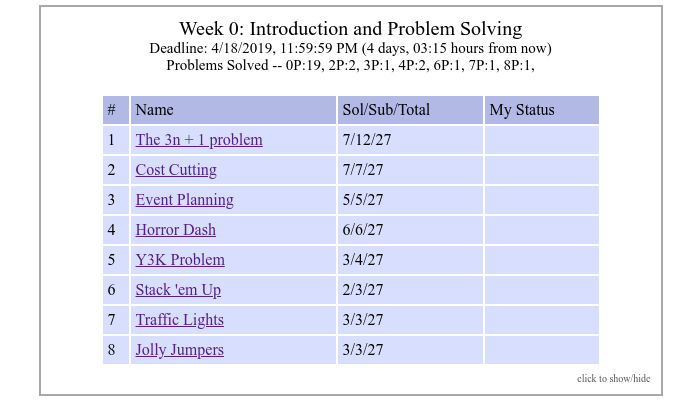
\includegraphics[width=0.9\textwidth]{img/resultsW0}
  \end{center}

  \begin{block}{}
    Very Good! It is going to get harder from here on.
  \end{block}
  
\end{frame}

\begin{frame}
  \frametitle{Today's Class: Solving Problems}
  \begin{block}{}
    Hints and ideas on how to solve programming challenges
  \end{block}

  \bigskip

  \begin{itemize}
  \item Reading Problems
  \item Considerations when programming
  \item Input/Output
  \item Debugging
  \item Types of Problems
  \end{itemize}
\end{frame}

\section{How to Solve Problems}
\subsection{Programming Challenge Workflow}
\begin{frame}
  \frametitle{A Programming Challenge Workflow}

  \begin{center}
    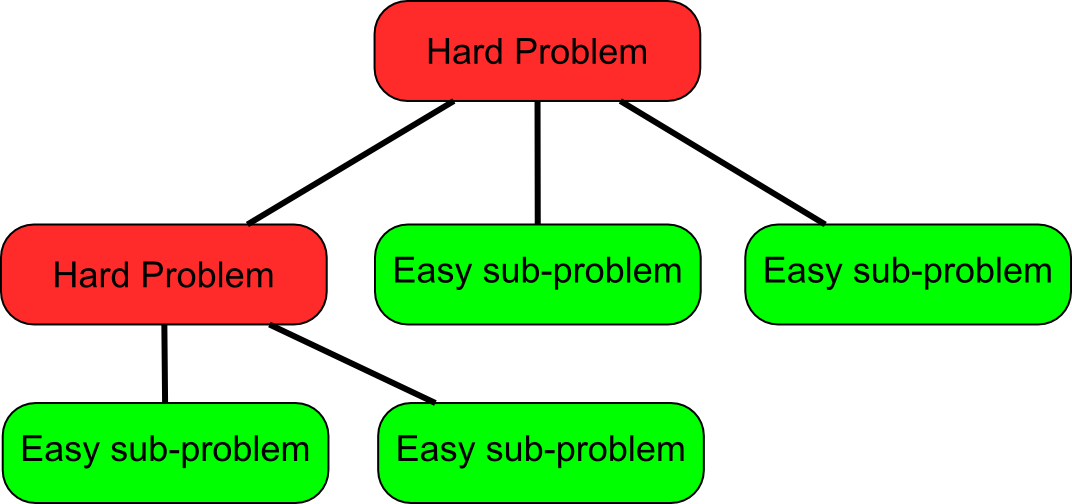
\includegraphics[width=0.5\textwidth]{../img/breakingtheproblem}
  \end{center}

  First trick of solving a hard problem: break it into simpler ones:
  
  {\smaller
  \begin{itemize}
  \item Task 1: Understand the problem description;
  \item Task 2: Understand the input/output;
  \item Task 3: Choose the Algorithm;
  \item Task 4: Write the Code;
  \item Task 5: Test the program on example data;
  \item Task 6: Test the program on hidden data;
  \end{itemize}}
\end{frame}

\subsection{Task 1: Reading The Problem}
\begin{frame}
  \frametitle{Task 1: Understanding the Problem Description}

  The English description is so hard!
  
  \bigskip

  \begin{block}{Don't Worry:}
  \begin{enumerate}
  \item Separate the text into \structure{flavor} and \structure{rules};
  \item Sometimes it is easy to read the input/output first, and then
    the text;    
  \item Problems with a lot of \structure{flavor} are usually not very hard.;
  \end{enumerate}
  \end{block}
\end{frame}

\begin{frame}
  \frametitle{Example: Problem 11559 -- Event Planning}

  {\smaller
  \begin{alertblock}{Flavor:}
    As you didn't show up to the yearly general meeting of the Nordic
    Club of Pin Collectors, you were unanimously elected to organize
    this years excursion to Pin City.  You are free to choose from a
    number of weekends this autumn, and have to  nd a suitable hotel
    to stay at, preferably as cheap as possible.
  \end{alertblock}

  \begin{exampleblock}{rules}
    You have some \underline{constraints}: The total \underline{cost}
    of the trip must be within \underline{budget}, of course. All
    participants \underline{must stay at the same hotel}, to avoid
    last years catastrophe, where some members got lost in the city,
    never being seen again.
  \end{exampleblock}

  \bigskip

  {\bf Keywords:} constraints, minimum, maximum, cost, rules, number,
  etc...  }
\end{frame}


\begin{frame}
  \frametitle{Extreme example: UVA 1124, Celebrity Jeopardy}
  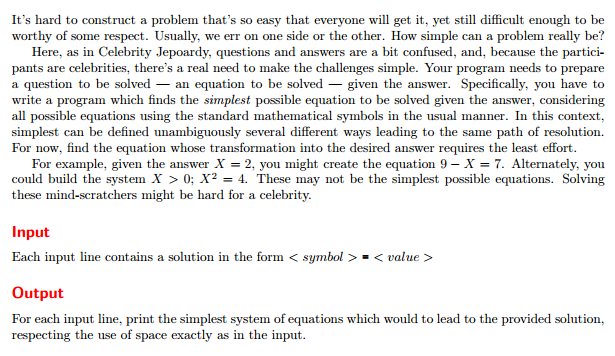
\includegraphics[width=0.9\textwidth]{../img/celebrityjeopardy}

  \hrulefill\\
  \alert{Real Problem:}
  Copy the input into the output. (look at the examples)
\end{frame}

\begin{frame}
  \frametitle{Hints for hard to read problems}
  
  \begin{columns}
    \column{0.7\textwidth}
    {\small
    \begin{itemize}
    \item If it is hard, look at the examples;
    \item If it is really hard, print on paper;
    \item First read: mark keywords;
    \item Second read: cut flavor;
    \item Re-write the important parts in another file;
    \item \alert{Do not begin programming until you understand the problem!}
    \end{itemize}
    }
    \column{0.3\textwidth}
    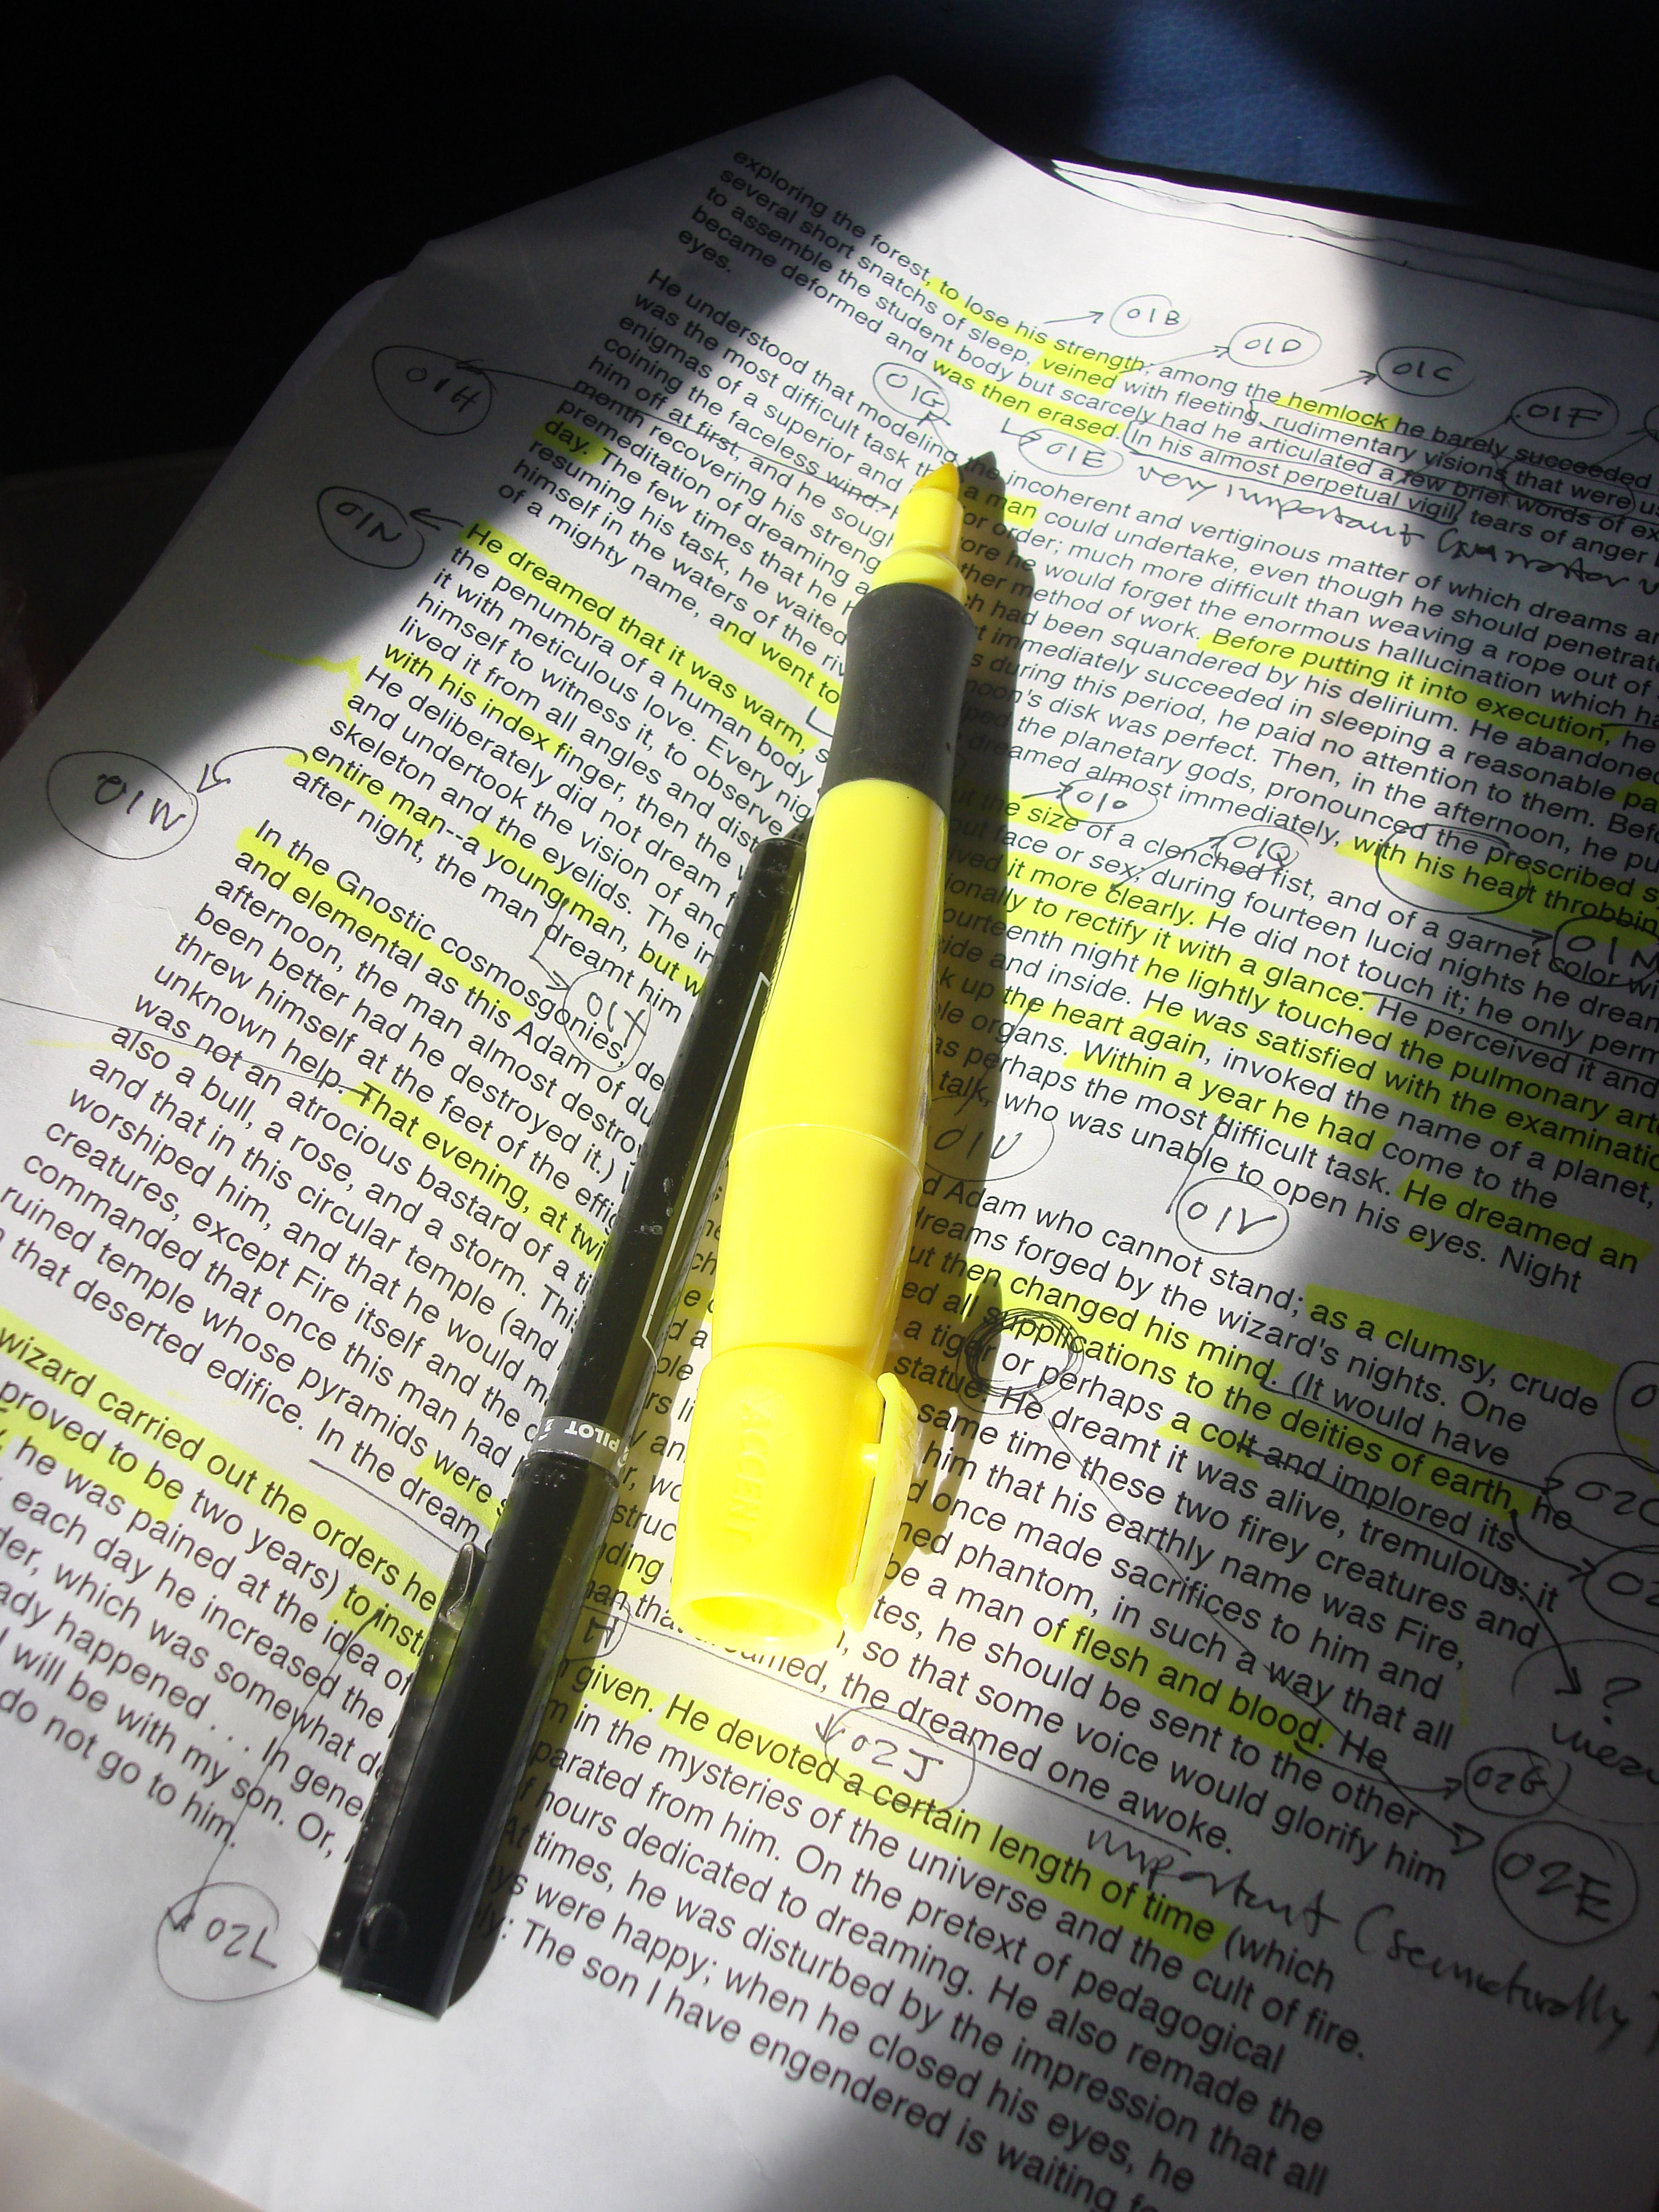
\includegraphics[width=\textwidth]{../img/textmarker}
  \end{columns}

  \vfill

  \hrulefill\\
  \hfill {\tiny Image by Guido ``random'' Alvarez, released as CC-BY-2.0}

\end{frame}

\subsection{Task 2: Understanding the Input/Output}

\begin{frame}
  \frametitle{Task 2: Understanding the Input}

  When you read the input, pay attention to:
  
  \bigskip

  {\small
  \begin{itemize}
  \item What is the problem size?
  \item What is the end condition?
  \item What type of data is it?
  \item What is the format of the data?
  \end{itemize}
  }
\end{frame}

\begin{frame}
  \frametitle{Task 2: Input Size}

  The input size shows how big the problem gets.

  \begin{itemize}
  \item If the problem is too small, you can try a brute force
    algorithm;
  \item If the problem is too big, you must use a more complex
    algorithm;
  \end{itemize}
  
  \begin{block}{Keep in Mind!}
    \begin{itemize}
    \item The average time limit in UVA is 1-3 seconds.
    \item Assume around 10.000.000 operations per second (in the judge).
    \item Use this as a \alert{rough measure} of time your program spends.
    \end{itemize}
  \end{block}
\end{frame}

\begin{frame}
  \frametitle{Task 2: Input Size -- Examples}

  \begin{block}{n $<$ 24}
    Exponential algorithms will work (O($2^n$)).\\
    Or sometimes you can just calculate all solutions.
  \end{block}

  \begin{block}{n = 500}
    Cubic algorithms don't work anymore (O($n^3$) = 125.000.000)\\
    Maybe O($n^2\text{log}n$) will still work.
  \end{block}

  \begin{block}{n = 10.000}
    A square algorithm (O($n^2$)) might still work.\\
    But beware any big constants!
  \end{block}

  \begin{block}{n = 1.000.000}
    O($n$log$n$) = 13.000.000\\
    We might need a linear algorithm!
  \end{block}
\end{frame}

\begin{frame}
  \frametitle{Task 2: Input Types}

  You should pay attention to the \structure{type and format} of the
  input.

  \vfill

  \begin{itemize}
  \item Reading A fixed number of tokens;
  \item Reading Until a condition;
  \item Reading until the end of the input;
  \end{itemize}
\end{frame}

\begin{frame}[fragile]
  \frametitle{Task 2: Input Types}
  \begin{block}{Reading a fixed number of tokens}
    The first line of the input says the total number of
    tokens/lines/cases to read;
  \end{block}

{\smaller 
\begin{verbatim}
#include <iostream>
using namespace std;

int main()
{
    int n;    
    cin >> n;

    for (; n > 0; n--)
    {
       // Do something
    }    
}
\end{verbatim}}

\end{frame}

\begin{frame}[fragile]
  \frametitle{Task 2: Input Types}
  \begin{block}{Conditional Ending}
    The problem specifies a special case to end the input.
  \end{block}

  \bigskip

  \structure{Example -- Request for Proposal:}\\
  The input ends with a line containing two zeroes.
  
{\smaller
\begin{verbatim}
int main()
{
   cin >> n >> p;
   cin.ignore(1000, '\n'); 
   // throws away the \n for a future getline
   while (n!=0 || p!=0)
   {
       // do something!
       cin >> n >> p;               
       cin.ignore(1000, '\n');
   }
}
\end{verbatim}}
\end{frame}

\begin{frame}[fragile]
  \frametitle{Task 2: Input Types}
  \begin{block}{Reading until the end of file}

    Put your reading function (getline, cin) inside a conditional.
    The input goes on until the end of the file. No explicit
    terminating value.\\ \structure{Example:} 100 -- The N+1 Problem
  \end{block}
{\smaller
\begin{verbatim}
#include<string>
int main()
{
    int a, b;
    while (cin >> a >> b;)
    {
        // Do something!
    }
}
\end{verbatim}
}
\end{frame}

\begin{frame}
  \frametitle{Reading the Output -- Correctness}

  The UVA judge will evaluate your code based on a simple \emph{diff}. 
  Be \alert{very careful} to write your output exactly like stated.

  \vfill

  \begin{columns}
    \column{0.2\textwidth}
    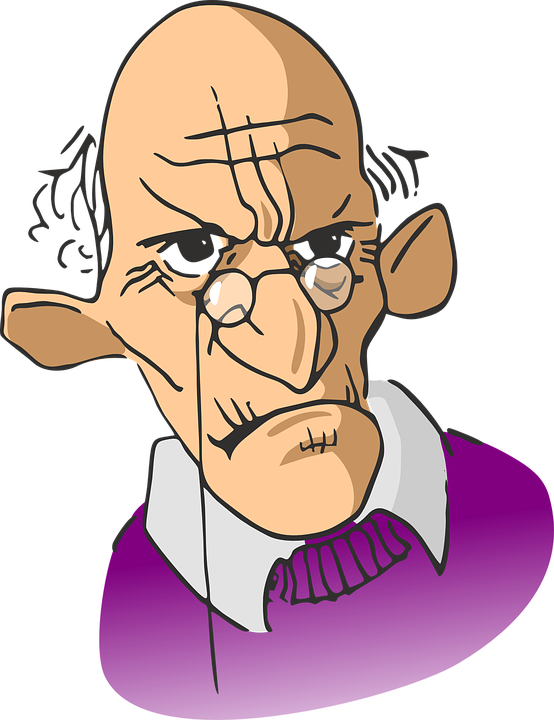
\includegraphics[width=1\textwidth]{../img/angryclient}
    \column{0.7\textwidth} \emph{The Judge is like an angry client. It
      wants the output EXACTLY how it stated.}
  \end{columns}
\end{frame}

\begin{frame}
  \frametitle{Easy to Miss errors in the output}

  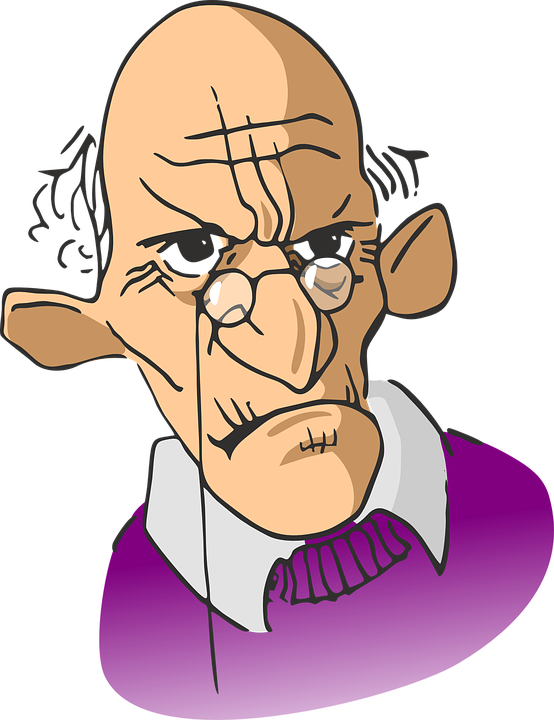
\includegraphics[width=0.15\textwidth]{../img/angryclient}
  \begin{itemize}
  \item Are the words uppercase, or lower case? (Case \structure{or} case)
  \item Are there any mistakes in the words? (case \structure{or} caes)
  \item Singular or plural? (1 hours \structure{or} 1 hour)
  \item What is the precision of floating numbers? (3.051 \structure{or} 3.05)
  \item Do you round up or round down? (3.62 $\rightarrow$ 3 \structure{or} 4)
  \item Is there more than one answer?
  \end{itemize}
\end{frame}


\begin{frame}
  \frametitle{Reading the problem: Identify Traps!}

  Be very careful to find traps in the problem:

  \vfill
  
  \begin{block}{Example: 3n+1 Problem}
    \begin{itemize}
    \item The two numbers $i$ and $j$ in the input can come in any
      order.
    \item But the output must be in the same order as the input!
    \end{itemize}
  \end{block}
    
  \vfill

  \hfill 
\includegraphics[width=0.25\textwidth]{../img/trap}
\end{frame}

\begin{frame}
  \frametitle{Reading the problem: Identify Traps!}


  \begin{block}{Common Traps}
    \begin{itemize}
    \item Negative numbers, zeros;
    \item Duplicated input, empty input;
    \item No solutions, multiple solutions;
    \item Other special cases;
    \end{itemize}
  \end{block}

  \hfill 
\includegraphics[width=0.25\textwidth]{../img/trap}
\end{frame}

\subsection{Task 3: Choosing the algorithm}

\begin{frame}
  \frametitle{Task 3: Choosing the algorithm}
  \begin{block}{3.1 What type of problem it is?}
    \begin{itemize}
    \item {\bf Full Search:} Tests all possible solutions;
    \item {\bf Greedy:} Break the solution, and try each best subsolution;
    \item {\bf Simulation:} Execute a series of steps, record the results;
    \item {\bf Dynamic Programming:} Table of partial solutions;
    \item {\bf Counting:} Calculate the number of possible solutions;
    \item {\bf Ad-hoc:} No fixed category;
    \item And many others;
    \end{itemize}
  \end{block}

  \bigskip

  First understand the problem; Then think; \alert{lastly code}.
\end{frame}

\begin{frame}
  \frametitle{Task 3: Choosing the algorithm}
  Basic considerations for recursive and iterative algorithms:

  \begin{itemize}
  \item An algorithm with k-nested loops of about n iterations each
    has O(nk) complexity;
  \item A recursive algorithm with b recursive calls per level, and L
    levels, it should have O(bL) complexity;
  \item Use pruning to reduce the complexity of algorithms.
  \item An algorithm processing a $n*n$ matrix in O(k) per cell runs
    in $O(kn^2)$ time. 
  \end{itemize}
\end{frame}

\begin{frame}
  \frametitle{Task 3: Choosing the algorithm}
  
  Example of Pruning: The 8-queen problem

  \vfill
  
  \begin{block}{Pruning with a good data structure}
    \begin{itemize}
    \item 8x8 matrix, with 1 for each queen: 64*63*62... = 1.78e+14
    \item 1 queen per column: 8*8*8*... = 1.67+e8
    \item 1 queen per column/row: 8*7*6... = 40320
    \end{itemize}
  \end{block}

  \bigskip

  You can prune even more by removing simmetries!
\end{frame}

\subsection{Task 4: Coding}

\begin{frame}
  \frametitle{Task 4: Coding}

  Do you understand \structure{The Problem} and \structure{The Algorithm}?

  \bigskip

  {\bf NOW} you can start writing your program.

  \vfill

  \begin{block}{}
    If you start your program before you understand the solution, you
    will create many more bugs.
  \end{block}
\end{frame}

\begin{frame}
  \frametitle{Task 4: Coding}
  \begin{exampleblock}{Hint 1: ``The Library''}
    Create a file with code examples that you often use.
    \begin{itemize}
    \item Input/output functions;
    \item Common data structures;
    \item Difficult algorithms;
    \end{itemize}
   \end{exampleblock}

   \begin{block}{Hint 2: Use paper}
    \begin{itemize}
    \item Writing your idea on paper help you visualize;
    \item Sometimes you can find bugs this way;
    \end{itemize}
  \end{block}
\end{frame}

\begin{frame}
  \frametitle{Task 4: Coding} 

  \begin{block}{Hint 3: Programmer Efficiency}
    Everyone knows about \structure{CPU efficiency} or
    \structure{Memory efficiency}.

    \bigskip

    But \structure{Programmer Efficiency} is very important too: Don't
    get \structure{tired/confused!}
  \end{block}

  \vfill
  
  \begin{itemize}
  \item Use standard library and macros;
  \item Your program just need to solve THIS problem;
  \item Use simple structures and algorithms;
  \item TDD mindset;
  \end{itemize}
\end{frame}


\subsection{Testing}
\begin{frame}
  \frametitle{Task 5,6: Test and Hidden Data}

  The example data {\bf is not} all the data!
  
  \bigskip

  \begin{columns}
    \column{0.45\textwidth}
    \begin{exampleblock}{Example Data}
      \begin{itemize}
      \item Useful to test input/output;
      \item Read the example data to understand the problem;
      \end{itemize}
    \end{exampleblock}
    \column{0.45\textwidth}
    \begin{alertblock}{Hidden Data}
      \begin{itemize}
      \item Used by the UVA judge;
      \item Contain bigger data sets;
      \item Includes special cases;
      \end{itemize}
    \end{alertblock}
  \end{columns}
  
  \medskip

  Generate your own set of hidden data before submitting!
\end{frame}

\begin{frame}
  \frametitle{What data to generate?}

  \begin{itemize}
  \item Datas with multiple entries (to check for initialization);
  \item Datas with maximum size (can be trivial cases);
  \item Random data;
  \item Border cases (maximum and minimum values in input range);
  \item Worst cases (depends on the problem);
  \end{itemize}
\end{frame}

\begin{frame}
  \frametitle{The uDebug Website}

  \begin{center}
    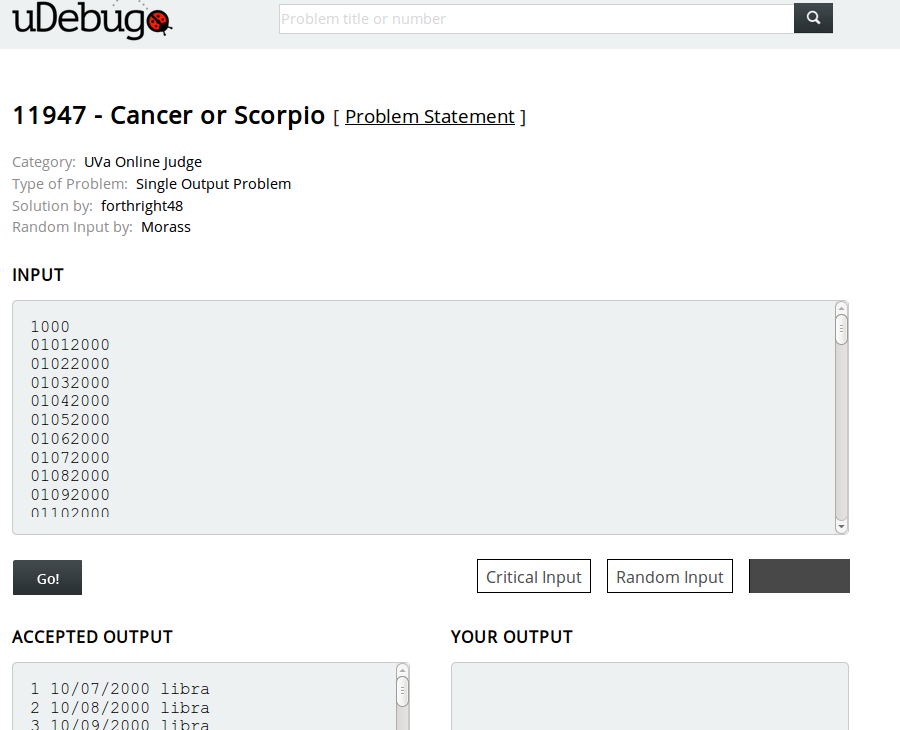
\includegraphics[width=0.8\textwidth]{../img/udebug_big}
  \end{center}
\end{frame}

\section{Conclusion}
\subsection{The End}
\begin{frame}
  \frametitle{To Summarize}
  Mental framework to solve problems:
  \begin{enumerate}
  \item Read the problem carefully to avoid traps;
  \item Think of the algorithm and data structure;
  \item Keep the size of the problem in mind;
  \item Keep your code simple;
  \item Create special test cases;
  \end{enumerate}

  \vfill

  \begin{block}{}
    Now go solve the other problems!
  \end{block}
\end{frame}

\begin{frame} 
  \frametitle{Thanks for Listening!}
  \begin{center}
    Any questions?
  \end{center}
\end{frame}

\begin{frame}
  \frametitle{BONUS I -- The most expensive program ever?}

  \begin{block}{Ackermann's Function}
    \begin{eqnarray*}
      A(m,n) = & n+1 & \text{if } m = 0\\
      & A(m-1,1) & \text{if } m > 0, n = 0\\
      & A(m-1,A(m,n-1)) & \text{if } m > 0, n > 0\\
    \end{eqnarray*}
  \end{block}
  
  \begin{itemize}
    \item $A(0,n) = n+1$
    \item $A(1,n) = n+3$
    \item $A(2,n) = 2n+3$
    \item $A(3,n) = 2^{n+3}-3$ \alert{!}
    \item $A(4,n) = 2^{2^{...^2}}-3$ \alert{!!!} (exponential tower of n+3)
    \item $A(5,n) = $ \alert{!!!!!!!!!!!!}
  \end{itemize}
\end{frame}

\begin{frame}
  \frametitle{BONUS II -- Typing Fast}  

  Practice typing in one of many online typing challenges.
  \begin{itemize}
  \item \url{www.typingtest.com}
  \item \url{https://typing.io} -- for programmers!
  \end{itemize}    
\end{frame}

% TODO Find info about 2017 ICPC

%\begin{frame}
%  \frametitle{BONUS II -- More Info on the ICPC Programming Challenge}
%  \begin{itemize}
%  \item Application deadline: 06/10 (Fri) -- 3-people team
%  \item Internet based contest: 06/24 (Fri) -- At Tsukuba
%  \item Webpage: \url{http://icpc.iisf.or.jp/2015-tsukuba/?lang=ja}
%  \end{itemize}
%  \bigskip

%  Ask me for details!
%\end{frame}

\end{document}
